\chapter{局部整体原理、阿代尔与伊代尔}\label{L3}
\lecturedate{2020/02/24}
\sourcepage{19}
\section{局部整体原理}\label{L3S1}\idx{局部整体原理}
在定义阿代尔与伊代尔之前，先介绍局部整体原理。

数论关注的主要问题之一，是求多项式方程$P(x_1,\ldots,x_n)=0$的整数解，例如Fermat大定理所涉及的方程。不过，较容易判定的问题是是否存在“模$m$”的整数解，即
\[P(x_1,\ldots,x_n)\equiv0\pmod m.\]
此外，对任意素数$p$，对所有$k\in\Z_{>0}$，同余式$P(x_1,\ldots,x_n)\equiv0\pmod{p^k}$都有解，等价于$P(x_1,\ldots,x_n)=0$在$\Z_p$中可解。对于二次齐次多项式方程，有如下称为“局部整体原理”\znote{局部整体原理问的是：一个整体对象若在每个素位处都有局部解，能否由此断定它有整体解。Hasse--Minkowski 定理说二次型情形答案为「是」；但对次数不低于 $3$ 的方程一般不成立，局部可解只是必要条件，因此它是一类需要逐情形验证的现象，而非普遍方法。[来源：Neukirch, \textit{Algebraic Number Theory}, Grundlehren der mathematischen Wissenschaften 322, 第 VI 章（本讲参考文献）。]}的定理。
\originalnumber{1}
\begin{theorem}{Hasse--Minkowski}\label{L3S1O1}\idx{Hasse--Minkowski定理}
给定二次型$Q(x_1,\ldots,x_n)=\sum_{i,j=1}^n a_{ij}x_ix_j$，其中$(a_{ij})$为整数对称矩阵，且$\det(a_{ij})\ne0$。方程$Q(x_1,\ldots,x_n)=0$有非平凡整数解，当且仅当它有非平凡实数解，并对每个$p$都有非平凡$p$进解。
\end{theorem}
这里，$\R$是$\Q$关于阿基米德素位——绝对值$|\cdot|$——的完备化。把$\R$看作$\Q$在“无穷素位”处的完备化时，也记为$\Q_\infty$。\eref{定理}{L3S1O1}指出：$\Q$上的二次型有整体解，即$\Q$中的非平凡解，
\sourcepage{20}
当且仅当它在包括无穷素位在内的所有素位$p$处都有非平凡局部解。

局部整体原理与本课程并无很直接的关系，但它提示我们：如果把所有局部对象置于同等地位，整体对象或许能由其局部数据确定。设$F$为数域，$\OO_F$为其代数整数环。相对于在各素位处完备化所得的局部域$F_{\p}$，我们称$F$为整体域\znote{整体域指 $\Q$ 的有限扩张（数域）或 $\F_q(t)$ 的有限扩张（函数域）。与只看一个素位的局部域相对，整体域同时记住全部素位的算术；数域 $F$ 沿对角线嵌入 $\prod_{\p}F_{\p}$，其像离散，这使得「用全部局部数据刻画整体对象」成为可能。[来源：Neukirch, \textit{Algebraic Number Theory}, Grundlehren der mathematischen Wissenschaften 322, 第 VI 章（本讲参考文献）。]}。研究与$F$有关的对象时，可以为每个$F_{\p}$定义相应的局部对象，进行分析，并尝试寻找某种局部整体原理；尤其当局部对象可能更容易处理时，这样做很自然。

现在我们要描述$\Gal(F^{\mathrm{ab}}/F)$，因此考察$F$的所有素位处的$\Gal(F_{\p}^{\mathrm{ab}}/F_{\p})$。对域$K$，记$K^\times$为非零元素组成的乘法群。
\begin{enumerate}
\item 若$\p$为无穷素位，则$\overline F_{\p}=\C$，$F_{\p}=\R$或$\C$。因此$\Gal(\overline F_{\p}/F_{\p})$或为平凡群，或为二阶循环群。
\item 若$\p$为有限素位，则$F_{\p}$是带离散赋值的局部域\znote{局部域是「只用一个素位的显微镜看数域」所得的对象：完备化 $F_{\p}$ 保留 $\p$ 处的分歧与剩余域，却丢掉了其它素位的信息。非阿基米德局部域即 $\Q_p$ 或 $\F_q((t))$ 的有限扩张，其整数环是离散赋值环；阿基米德局部域只有 $\R$ 与 $\C$。[来源：Neukirch, \textit{Algebraic Number Theory}, Grundlehren der mathematischen Wissenschaften 322, 第 V 章（本讲参考文献）。]}。一般而言，$\Gal(\overline F_{\p}/F_{\p})$尚未被充分理解，但有限Galois扩张$L_{\Pp}/F_{\p}$的群$\Gal(L_{\Pp}/F_{\p})$有许多良好性质。此外，局部类域论给出$F_{\p}$的有限阿贝尔扩张与$F_{\p}^\times$的范数子群之间的一一对应。
\end{enumerate}
设$L/F$为有限Galois扩张，$D$为$\OO_F$在$L$中的整闭包。设$\Pp$为$L$中位于$F$的素位$\p$上方的素位。回忆，$\Pp$的分解群为
\[G_{\Pp}=\{\sigma\in\Gal(L/F)\mid\sigma\Pp=\Pp\}.\]
当$\p$为无穷素位时，它对应于$F$到$\R$或$\C$的嵌入（模去复共轭），$\Pp$则是这一嵌入到$L$的延拓。记此延拓为$\iota_{\Pp}$，则
\[G_{\Pp}=\{\sigma\in\Gal(L/F)\mid\iota_{\Pp}\circ\sigma=\iota_{\Pp}\text{ 或 }\overline\iota_{\Pp}\}.\]
% [Tutor Note: 原书 p20 的分解群条件只写 ι_P∘σ = ι_P；当 p 为实素位而 P 为复素位时，还应允许 ι_P∘σ 等于 ι_P 的共轭，译文按完整条件处理。]
我们知道$L_{\Pp}/F_{\p}$为Galois扩张，因此每个$\sigma\in G_{\Pp}$都诱导$L_{\Pp}$的一个$F_{\p}$-自同构，得到映射$i:G_{\Pp}\longrightarrow\Gal(L_{\Pp}/F_{\p})$。
\sourcepage{21}
\originalnumber{2}
\begin{proposition}\label{L3S1O2}
$i:G_{\Pp}\longrightarrow\Gal(L_{\Pp}/F_{\p})$为同构。
\end{proposition}
\begin{proof}
由于$L\subseteq L_{\Pp}$，$i$为单射。只需证明$|G_{\Pp}|=|\Gal(L_{\Pp}/F_{\p})|$。对于有限素位，设$\p D=\Pp_1^e\cdots\Pp_r^e$，其中$f=[D/\Pp_j:\OO_F/\p]$；由Hilbert分歧理论，$efr=[L:F]$（见\lref{L2}\sref{L2S1}）。另一方面，由于$\Gal(L/F)$在$\{\Pp_1,\ldots,\Pp_r\}$上传递作用，$r=|\Gal(L/F)|/|G_{\Pp}|$。因此
\[|\Gal(L_{\Pp}/F_{\p})|=[L_{\Pp}:F_{\p}]=ef=\frac{[L:F]}r=|G_{\Pp}|.\]
% [Tutor Note: 原书 p21 证明中把 [L:F] 写作 [L:K]，而本节 K 另指局部域，应为 [L:F]；译文按 [L:F] 处理。]
\end{proof}
由\eref{命题}{L3S1O2}，可把每个$\Gal(L_{\Pp}/F_{\p})$看成$\Gal(L/F)$的子群。
\section{局部类域论}\label{L3S2}\idx{局部类域论}
下面简要回顾局部类域论的一些结论。设$K$为局部域，$v_K$为规范化的离散赋值（即$v_K:K^\times\longrightarrow\Z$为满射）。设$\OO_K$为$K$的整数环，它是离散赋值环，有唯一的非零素理想$\p$。记剩余域为$k=\OO_K/\p$，则$k\cong\F_q$为有限域。
% [Tutor Note: 原书 p21 作 $v_K:K\to\Z$ 为满射；赋值在 $0$ 处无定义，定义域应为 $K^\times$，译文按 $v_K:K^\times\to\Z$ 处理。]
\begin{property}
设$E$为$K$的有限扩张，$R$为$\OO_K$在$E$中的整闭包。则$E$也是局部域，$R$为离散赋值环，$\Pp$为其唯一的非零素理想。记$E$的剩余域为$k_E=R/\Pp$，则$k_E$是$k$的有限扩张。
\end{property}
\begin{definition*}{局部非分歧扩张}
有$\p R=\Pp^e$及$e[k_E:k]=[E:K]=:n$。若$e=1$，称$E$在$K$上\textbf{非分歧}。
\end{definition*}
\begin{property}
若$E/K$非分歧，则$E/K$为Galois扩张$\iff k_E/k$为Galois扩张；在此情形下，$\Gal(E/K)\cong\Gal(k_E/k)$。因此，非分歧扩张都是阿贝尔扩张。
\end{property}
\sourcepage{22}
对有限Galois扩张$E/K$，定义范映射
\[N_{E/K}:E^\times\longrightarrow K^\times,\qquad\alpha\longmapsto\prod_{\sigma\in\Gal(E/K)}\sigma(\alpha).\]
\originalnumber{1}
\begin{theorem}\label{L3S2O1}
设$E/K$为有限Galois扩张。存在局部互反映射
\[\theta:K^\times/N_{E/K}(E^\times)\xrightarrow{\sim}\Gal(E/K)^{\mathrm{ab}},\]
且此映射为同构。
\end{theorem}
\eref{定理}{L3S2O1}的证明从略。这里只指出，若$E/K$非分歧，则$\Gal(E/K)\cong\Gal(k_E/k)$为阿贝尔群，由Frobenius元素$\mathcal F$生成；映射$\widetilde\theta(\alpha)=\mathcal F^{v_K(\alpha)}$（$\alpha\in K^\times$）诱导$\theta$。等式$\ker\widetilde\theta=N_{E/K}(E^\times)$由下面的命题得出。
\originalnumber{2}
\begin{proposition}\label{L3S2O2}
设$U_K$、$U_E$分别为$\OO_K$、$R$的单位群。若$E/K$非分歧，则$N_{E/K}(U_E)=U_K$。
\end{proposition}
\begin{exercise*}\label{L3S2EX}
利用\eref{命题}{L3S2O2}，证明当$E/K$非分歧时，$\ker\widetilde\theta=N_{E/K}(E^\times)$。
\end{exercise*}
若子群$M\subseteq K^\times$可写成$M=N_{E/K}(E^\times)$，其中$E/K$为某个有限阿贝尔扩张，就称$M$为\textbf{范数子群}\znote{范数子群就是「能作为某个有限阿贝尔扩张的范数像」的乘法子群。局部类域论断言：$K^\times$ 的有限指数闭子群恰好都是范数子群。于是 $K$ 的有限阿贝尔扩张与这些子群一一对应，阿贝尔扩张的全部信息被编码进 $K^\times$ 的群论数据，这正是类域论的核心。[来源：Neukirch, \textit{Algebraic Number Theory}, Grundlehren der mathematischen Wissenschaften 322, 第 V 章（本讲参考文献）。]}。\idx{范数子群}
\originalnumber{3}
\begin{theorem}{Galois对应}\label{L3S2O3}
$K$的有限阿贝尔扩张与$K^\times$的范数子群之间存在一一对应。此外，
\[N_{E_1/K}(E_1^\times)\subseteq N_{E_2/K}(E_2^\times)\iff E_2\subseteq E_1.\]
\end{theorem}
\originalnumber{4}
\begin{note}[L3S2O4]
范数子群$M\subseteq K^\times$还有一个内在刻画：$M$为范数子群，当且仅当它是$K^\times$中有限指数的闭子群；这里$K^\times$赋予Krull 拓扑\idx{Krull拓扑}。
\end{note}
% [Tutor Note: 原书 p22 Remark 2.4 把局部域 $K$ 写作 $F_{\p}$，与该节记号不符；译文按 $K^\times$ 处理。]
\originalnumber{5}
\begin{note}[L3S2O5]
\eref{定理}{L3S2O1}也可包括阿基米德情形。若$K=\C$，没有需要证明的内容；若$K=\R$，唯一的非平凡有限阿贝尔扩张$\C$对应于子群$\R_{>0}\subseteq\R^\times$。
\end{note}
\section{阿代尔与伊代尔}\label{L3S3}\idx{阿代尔}\idx{伊代尔}
设$F$为整体域，$F_{\p}$为$F$关于素位$\p$（允许为无穷素位）的完备化。若$\p$有限，记其赋值环为$\OO_{\p}$。
\sourcepage{23}
对于无穷素位，取$\OO_{\p}=F_{\p}$，其中$F_{\p}=\R$或$\C$。记$F_{\p}$上的赋值为$v_{\p}$。
% [Tutor Note: 原书 p23 作「$\OO_{\p}=\R_{\ge0}$（当 $F_{\p}=\R$）」；$\R_{\ge0}$ 对加法不封闭、不是环，此处应为 $\OO_{\p}=F_{\p}=\R$，译文按正确写法处理。]

$F$的\textbf{阿代尔环}$\A_F$\znote{阿代尔环把 $F$ 在所有素位处的完备化同时收进一个环，使「对所有素位同时成立」的陈述有统一载体。对角嵌入 $F\hookrightarrow\A_F$ 把数域的元素变成阿代尔。整体不变量（伊代尔类群、自守形式、$L$ 函数）都定义在 $\A_F$ 或其商上，这是 Langlands 纲领的技术起点。[来源：Cassels--Fr\"ohlich, \textit{Algebraic Number Theory}, 第 II 章（本讲参考文献）。]}是无限直积$\prod_{\p}F_{\p}$的子环，由所有满足$\alpha_{\p}\in F_{\p}$、且除有限多个$\p$外均有$\alpha_{\p}\in\OO_{\p}$的元素$\alpha=(\alpha_{\p})_{\p}$组成；这里$\p$遍历$F$的所有素位，包括无穷素位。

$\A_F$中的加法、乘法逐分量定义。这种乘积称为各$F_{\p}$关于子环$\OO_{\p}\subseteq F_{\p}$的\textbf{限制直积}\znote{限制直积的拓扑比 $\prod_{\p}F_{\p}$ 的直积拓扑更细：$\prod_{\p}\OO_{\p}$ 在限制直积拓扑下是开集，在子空间拓扑下却不是。原因是直积拓扑的每个基本开集只允许有限多个分量异于 $F_{\p}$。这一差别使 $\A_F$ 局部紧，而无限直积不局部紧；讨论收敛时必须用限制直积拓扑。[来源：Cassels--Fr\"ohlich, \textit{Algebraic Number Theory}, 第 II 章（本讲参考文献）。]}。各分量的拓扑赋予$\A_F$限制直积拓扑，使其成为拓扑环，加法与乘法连续。$\A_F$还是局部紧的，因为各$F_{\p}$局部紧，且有限素位处的$\OO_{\p}$紧。\idx{限制直积}\idx{阿代尔环}

$F$的\textbf{伊代尔群}$\mathbb{I}_F$是阿代尔环中的单位群$\mathbb{I}_F=\A_F^\times$\znote{伊代尔群 $\mathbb{I}_F=\A_F^\times$ 由各分量都非零、且除有限多个素位外分量为单位的元素组成。换言之，它是 $\prod'_{\p}F_{\p}^\times$ 关于 $\OO_{\p}^\times$ 的限制直积。它把每个素位处的乘法信息一并携带；商掉主伊代尔 $F^\times$ 得到伊代尔类群，后者正是整体类域论与自守表示论工作的对象。[来源：Cassels--Fr\"ohlich, \textit{Algebraic Number Theory}, 第 II 章（本讲参考文献）。]}。换言之，它是各$F_{\p}^\times$关于$\OO_{\p}^\times$的限制直积。设$S$为素位的一个有限集合，则$\mathbb{I}_F^S$为$S$-伊代尔组成的子群，满足
\[\mathbb{I}_F^S=\prod_{\p\in S}F_{\p}^\times\times\prod_{\p\notin S}\OO_{\p}^\times.\]
各嵌入$F^\times\hookrightarrow F_{\p}^\times$诱导嵌入$F^\times\hookrightarrow\mathbb{I}_F$。注意，对每个$x\in F^\times$，满足$x\notin\OO_{\p}^\times$的$\p$只有有限多个。
\originalnumber{1}
\begin{definition}{伊代尔类群}\label{L3S3O1}\idx{伊代尔类群}
商群$\mathbb{C}_F:=\mathbb{I}_F/F^\times$称为$F$的\textbf{伊代尔类群}。
\end{definition}
$\mathbb{I}_F$赋予限制直积拓扑。在此拓扑下，$F^\times$是$\mathbb{I}_F$的离散子群。

回忆，在\lref{L2}中，我们用$I_F$表示$F$的分式理想群；$C_F:=C_1=I_F/i(F^\times)$则是理想类群。有满同态
\[(\ ):\mathbb{I}_F\longrightarrow I_F,\qquad\alpha\longmapsto(\alpha)=\prod_{\p\text{ 有限}}\p^{v_{\p}(\alpha_{\p})}.\]
\sourcepage{24}
映射$(\ )$的核为
\[\mathbb{I}_F^\infty=\prod_{\p\text{ 无穷}}F_{\p}^\times\times\prod_{\p\text{ 有限}}\OO_{\p}^\times.\]
因而有以下命题。
\originalnumber{2}
\begin{proposition}\label{L3S3O2}
映射$(\ )$诱导满射$\mathbb{C}_F\longrightarrow C_F$，其核为$\mathbb{I}_F^\infty F^\times/F^\times$。因此$C_F\cong\mathbb{I}_F/(\mathbb{I}_F^\infty F^\times)$。
\end{proposition}
对有限阿贝尔扩张$L/F$，结合\eref{命题}{L3S1O2}和\eref{定理}{L3S2O1}，可以定义整体互反映射$\theta:\mathbb{I}_F/N_{L/F}(\mathbb{I}_L)\longrightarrow\Gal(L/F)$。这里$N_{L/F}:\mathbb{I}_L\longrightarrow\mathbb{I}_F$定义为
\[N_{L/F}(\alpha^L)=\left(\prod_{\Pp\mid\p}N_{L_{\Pp}/F_{\p}}(\alpha^L_{\Pp})\right)_{\p}.\]
把每个$\Gal(L_{\Pp}/F_{\p})$看作$\Gal(L/F)$中的子群$G_{\Pp}=G_{\p}$，即可定义
\[\widetilde\theta:\mathbb{I}_F\longrightarrow\Gal(L/F),\qquad\widetilde\theta(\alpha)=\prod_{\p}\widetilde\theta_{\p}(\alpha_{\p}).\]
这个乘积有意义：对于在$L$中非分歧的$\p$，$\widetilde\theta_{\p}(\alpha_{\p})=\operatorname{Fr}[\p]^{v_{\p}(\alpha_{\p})}$；分歧的$\p$只有有限多个，且除有限多个$\p$外均有$v_{\p}(\alpha_{\p})=0$。$\widetilde\theta$诱导映射$\theta$。但$\theta$本身不是同构；有如下同样称为Artin互反律的定理。
\originalnumber{3}
\begin{theorem}{Artin互反律}\label{L3S3O3}
$F^\times\subseteq\ker\widetilde\theta$。换言之，$\displaystyle\prod_{\p}\widetilde\theta_{\p}(x)=1$，对所有$x\in F^\times$成立。
\end{theorem}
由\eref{定理}{L3S3O3}，得到映射$\overline\theta:\mathbb{C}_F/N_{L/F}(\mathbb{C}_L)\longrightarrow\Gal(L/F)$。一个并不平凡的事实是，$\overline\theta$实际上是同构。由此可以用伊代尔类的范数群参数化$F$的所有有限阿贝尔扩张。
\originalnumber{4}
\begin{theorem}\label{L3S3O4}
\begin{enumerate}
\item $\Gal(L/F)\cong\mathbb{C}_F/N_{L/F}(\mathbb{C}_L)$。
% [Tutor Note: 原书 p24 定理 3.4(1) 作 Gal(L/K)，K 未定义，应为 Gal(L/F)；译文按 Gal(L/F) 处理。]
\item 映射$L\longmapsto N_{L/F}(\mathbb{C}_L)$给出$F$的有限阿贝尔扩张与$\mathbb{C}_F$中有限指数闭子群之间的一一对应。此外，
\[L_1\subseteq L_2\iff N_{L_1/F}(\mathbb{C}_{L_1})\supseteq N_{L_2/F}(\mathbb{C}_{L_2}).\]
\end{enumerate}
\end{theorem}
\sourcepage{25}
最后说明局部与整体互反映射的相容性。定义$\iota_{\p}:F_{\p}^\times\hookrightarrow\mathbb{C}_F$，把$a_{\p}$映到仅在$\p$分量为$a_{\p}$、其他分量全为$1$的伊代尔的类。于是有以下命题。
\originalnumber{5}
\begin{proposition}\label{L3S3O5}
设$L/F$为有限阿贝尔扩张，$\p$为$F$的一个素位（允许为无穷素位），$\Pp$为$L$中位于$\p$上方的素位。则下图交换：
\begin{figure}[H]\centering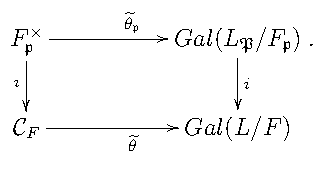
\includegraphics[width=0.2604\paperwidth]{images/L3-p025-diagram.pdf}\end{figure}
\end{proposition}
\eref{命题}{L3S3O5}表明，\eref{定理}{L3S3O4}中的同构$\overline\theta$满足某种刚性条件。
% [Tutor Note: 原书 p25 作「Theorem 3.3 中的同构 θ̄」，但 θ̄ 出现于 Theorem 3.4，Theorem 3.3 是 Artin 互反律；译文按定理 3.4 处理。]

\textbf{$n=1$时的Langlands纲领。}由无限Galois理论，
\begin{align*}
\Gal(F^{\mathrm{ab}}/F)&=\varprojlim_{L/F\text{ 有限阿贝尔}}\Gal(L/F)\\
&=\varprojlim_{N\text{ 为有限指数闭子群}}(\mathbb{C}_F/N).
\end{align*}
因此$\Gal(F^{\mathrm{ab}}/F)\cong G$，其中$G$为$\mathbb{C}_F$的连通分支群。

至此，我们完成了阿贝尔情形，即$n=1$时的Langlands纲领。对于一般$n$，Langlands纲领研究的不是Galois群$\Gal(\overline F/F)$本身，而是它的$n$维表示，即群同态$\sigma:\Gal(\overline F/F)\longrightarrow\GL_n$。它猜想存在如下的一一对应：
\[\left\{\begin{array}{c}\Gal(\overline F/F)\text{ 的}\\n\text{ 维表示}\end{array}\right\}\quad\overset{1\text{--}1}{\longleftrightarrow}\quad\left\{\begin{array}{c}\GL_n(\A_F)\text{ 的}\\\text{自守表示}\end{array}\right\}.\]
接下来的一两讲将定义自守表示，并考察$n=2$、$F=\Q$的非阿贝尔情形。
\needspace{5\baselineskip}\section{第3讲参考文献}\label{L3S4}
\needspace{4\baselineskip}关于局部类域论：
\sourcepage{26}
\begin{references}
\refitem{L3refN5}{N} J. Neukirch, \textit{Algebraic number theory}, Grundlehren der mathematischen Wissenschaften 322, Springer-Verlag Berlin Heidelberg GmbH, Chapter V.
\refitem{L3refCF6}{CF} J. W. S. Cassels and A. Fr\"ohlich, \textit{Algebraic Number Theory}, Proceedings of an instructional conference organized by the LMS, Chapter VI.
\end{references}
\needspace{4\baselineskip}关于阿代尔与伊代尔：
\begin{references}
\refitem{L3refN6}{N} J. Neukirch, \textit{Algebraic number theory}, Grundlehren der mathematischen Wissenschaften 322, Springer-Verlag Berlin Heidelberg GmbH, Chapter VI.
\refitem{L3refCF2}{CF} J. W. S. Cassels and A. Fr\"ohlich, \textit{Algebraic Number Theory}, Proceedings of an instructional conference organized by the LMS, Chapter II.
\end{references}
\needspace{4\baselineskip}关于伊代尔表述的Artin互反律：
\begin{references}
\refitem{L3refN6b}{N} J. Neukirch, \textit{Algebraic number theory}, Grundlehren der mathematischen Wissenschaften 322, Springer-Verlag Berlin Heidelberg GmbH, Chapter VI.
\refitem{L3refCF7}{CF} J. W. S. Cassels and A. Fr\"ohlich, \textit{Algebraic Number Theory}, Proceedings of an instructional conference organized by the LMS, Chapter VII.
\end{references}
